\chapter{Design and Implementation - Benchmarking}
\label{chapter:Design and Implementation - Benchmarking}
 
\section{Benchmarking: HBase vs MySQL}

In this section we compare our tuned HBase cluster against a standard MySQL cluster.

\bigskip

The benchmarking is based on a industry standard benchmark: Yahoo! Cloud Serving Benchmark (YCSB). For more information about this tool head to Background section: YCSB.
\par
The purpose of this benchmark is to compare HBase against MySQL in a variety of different scenarios, such as a heavy-write scenario or a heavy-read scenario. 
\par
YCSB works with its own data, which is represented as a table of records. Each record has a unique key and an amount of fields which represent record values. Despite it does not allow users to load their own data, YCSB data is really configurable in terms of how many records user wants, how many fields has each record and the size of them. So although we can not play with the prior real data, we can almost reproduce it. Our HBase table looks really similar to the used in the whole experiment, it has the same number of fields and the size of each field is the average size of our real data fields. BloomFilters, In\_Memory and blocksize properties are enable as in our experiments. The rest of HBase parameters looks like the ones we discussed earlier.
\par
The MySQL cluster has been compiled and subsequently deployed onto Triton with the same characteristics we have used for our HBase cluster deployment (Allocated RAM, Xeon nodes, etc). Therefore, our MySQL cluster is composed of five nodes and the data is spread evenly among them using a simple sharding function S(key), S = hash(key) \% numberOfNodes, because by default MySQL has no built-in clustering capabilities as HBase has. The MySQL table looks exactly like the HBase table does; ten fields by row, size of each one is the average size of our real data. InnoDB is used as the storage engine of our MySQL database and the row key is indexed by a B-Tree. 

\bigskip

DISCLAIMER: No MySQL-related parameters have been tuned for the benchmarks, but \textit{innodb\_buffer\_pool\_size} increased from 8MB to 3027MB. It is a storage area for caching data and indexes in memory. Also a B-Tree index is created on the row key of our table to enhance the query execution time. The rest of parameters continue as by default.

\bigskip

In the conducted benchmarks all fields are always read, the number of operations is always one million and the records to operate on follow a uniform distribution in order to be as close as possible to our real scenario fully described in the previous chapters. Table 7.1 summarizes the kinds of workload that we chose for benchmarking.

\begin{table}[htbp]

\begin{center}
\begin{tabular}{|l|l|l|l|}
\hline
Workload & Insert \% & Read \% & Update \% \\ \hline
Data Load & \multicolumn{1}{r|}{100} &  &  \\ \hline
Predominant Reads &  & \multicolumn{1}{r|}{95} & \multicolumn{1}{r|}{5} \\ \hline
Reads mixed with Updates &  & \multicolumn{1}{r|}{50} & \multicolumn{1}{r|}{50} \\ \hline
\end{tabular}
\caption{YCSB Workloads}
\end{center}

\label{Table YCSB Workloads.}
\end{table}

\par
Below we present results for each workload: load, predominant reads and reads with updates.

%http://www.pdl.cmu.edu/PDL-FTP/Storage/socc2011_abs.shtml

\subsection{Load phase}


\begin{figure}[htb]
\centering
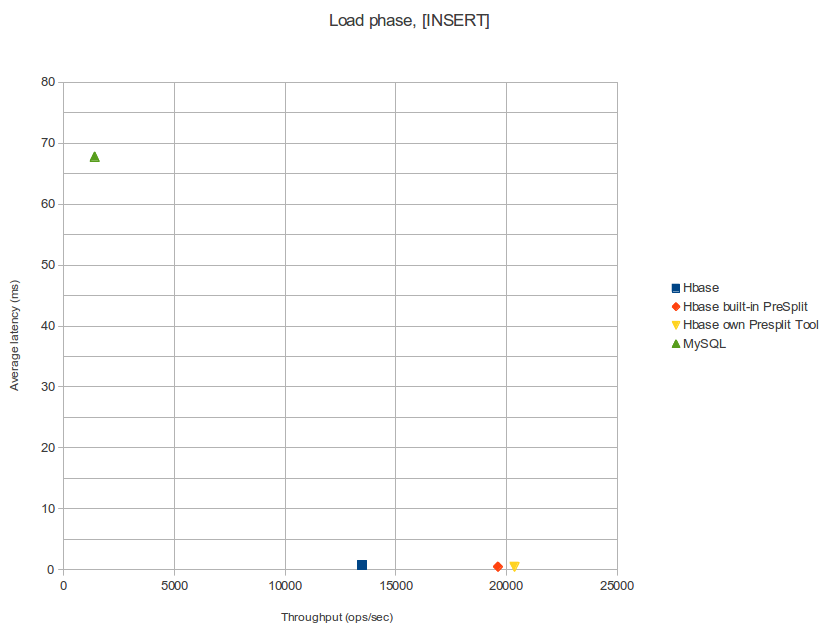
\includegraphics[width=1\textwidth]{./images/load.png}
 \label{fig:load}
\caption{Latency vs throughput comparison.}
\end{figure}


Along with the MySQL outcome, three different versions of HBase loads (see Figure 7.1) are depicted due to the lack of pre-split regions YCSB comes with. The first one, \textit{HBase} label, shows the default behaviour of YCSB, which is a table with only one region at the beginning. The other two correspond to different split region algorithms we have tested. The first, \textit{HBase built-in PreSplit} label, is based on the \textit{HBase.util.RegionSplitter} tool which allows users to create tables with a specified number of pre-split regions, assuming keys are uniformly distributed bytes. This tool gives out a much better performance than the \textit{HBase} version without pre-split regions. However, this can be improved a bit more because of the fact that YCSB does not export uniformly distributed bytes keys. Instead, it creates keys which are a combination of the string \textit{user} and a long integer (Ex. "user111111111111111").
\par
Once we understood the YCSB key-creation pattern, we developed a custom lightweight \textit{RegionSplitter} tool which leverages the YCSB key specification and creates a table with pre-split regions whose split points fits with the keys that YCSB will randomly create during the load phase. This tool, \textit{HBase PreSplit Tool} label, overcomes the previous results by achieving 20356 operations per second,  66.25\% better compared to the YCSB default throughput behavior (\textit{HBase} label). 
\par
We conclude that our tuned HBase cluster has unconquerable superiority in writes while MySQL is really far away from the HBase results.



\subsection{Reads mixed with Updates}


\begin{figure}[htb]
\centering
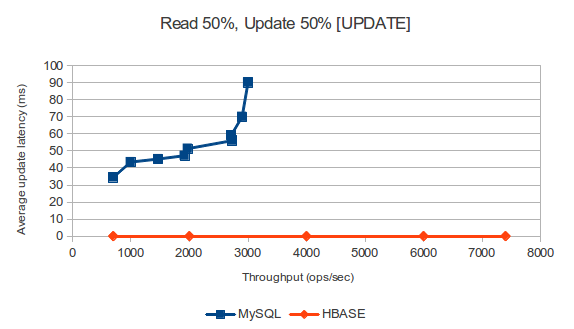
\includegraphics[width=1\textwidth]{./images/workloadAUpdate1.png}
\caption{Workload 50\% read 50\% update - Update.}
\label{fig:AUpdate}
\end{figure}

\begin{figure}[htb]
\centering
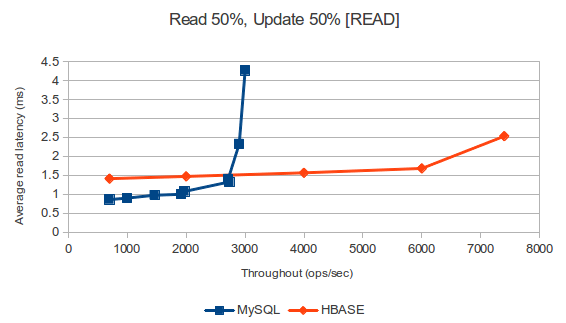
\includegraphics[width=1\textwidth]{./images/workloadARead1.png}
\caption{Workload 50\% read 50\% update - Read.}
 \label{fig:ARead}
\end{figure}

Figures 7.2 and 7.3 measures the latency/throughput curve of both HBase and MySQL clusters when dealing with a workload composed of 1.000.000 operations, 50\% are update operations and the other 50\% are read operations.
\par
HBase is optimized for writes and that is why it achieves higher throughput and lower latency than its competitor. The main reason of this performance is because edits are commited to memory firstly (WAL \textgreater\textgreater MemStore) and then aggregated edits are flushed to disk.


\subsection{Predominant Reads}

\begin{figure}[htb]
\centering
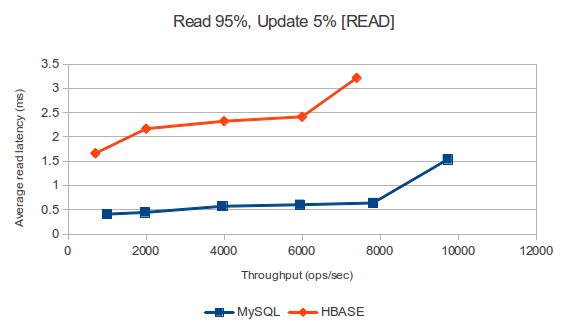
\includegraphics[width=1\textwidth]{./images/workloadBRead1.png}
\caption{Workload 95\% read 5\% - Read.}
 \label{fig:BRead}
\end{figure}

\begin{figure}[htb]
\centering
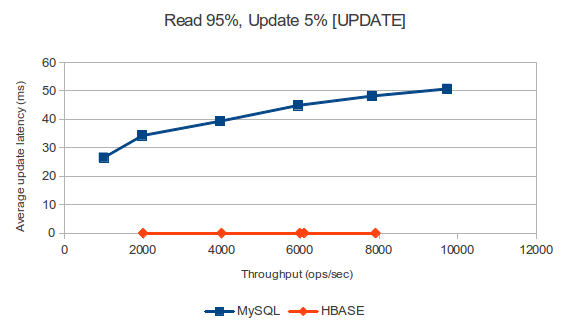
\includegraphics[width=1\textwidth]{./images/workloadBUpdate.png}
\caption{Workload 95\% read 5\% - Update.}
 \label{fig:BUpdate}
\end{figure}

Figures 7.4 and 7.5 measures the resulting latency/throughput curve of both HBase and MySQL clusters when dealing with a workload composed of 1.000.000 operations, 95\% of them are random reads and the 5\% rest are update operations.
\par
Upon studying the results we conclude that MySQL Sharded is a performance leader in reads. MySQL B-Tree indexes make the difference. Its only flaw is that it gets satured when the offered throughput reaches more than 9734 operations per second. Random read performance is slower in HBase because of the need to reconstruct records, but not much. Talking about Update, HBase results are from other world. MySQL has nothing to do against HBase when it comes to writes.














%http://www.academia.edu/2444832/Hybrid_HBase_Leveraging_Flash_SSDs_to_Improve_Cost_per_Throughput_of_HBase
























